\subsection{Detección de la cara y de los puntos faciales}
\label{sec:deteccion}

\textbf{Cara.} En el modo foto, la cara se ubica con el clasificador de Haar de OpenCV \cite{viola2001} (\archivo{detection/face_detector.py}) y se elige la de mayor área. En el modo en vivo no se usa, porque falló en el 30~\% de 2695 cuadros al girar la cabeza; ahí la cara sale directamente de los puntos.

\textbf{Puntos.} El modelo \emph{Face Landmarker} de MediaPipe \cite{kartynnik2019} devuelve 478 puntos normalizados con profundidad. Este modelo no lo entrenamos: se usa solo para inferencia. Como el resto del sistema se diseñó sobre el estándar iBUG de 68 puntos, \archivo{detection/landmarks.py} los convierte así:
\begin{itemize}
  \item \textbf{mandíbula}: los 23 puntos del contorno inferior se remuestrean por longitud de arco a 17 puntos equiespaciados (longitud acumulada e interpolación lineal);
  \item \textbf{cejas, ojos, nariz y boca}: 51 puntos salen de una tabla de correspondencias.
\end{itemize}
La malla completa con profundidad se conserva para el espejo 3D, el laboratorio y la forma de la cara.

\textbf{Estabilidad en vivo.} En video se usa el modo de seguimiento de MediaPipe y un filtro One-Euro \cite{casiez2012}. Es un pasa-bajos cuyo corte crece con la velocidad:
\begin{equation}
  f_c=f_{\min}+\beta\,|\hat{\dot x}|,\qquad \alpha=\frac{1}{1+\tau/\Delta t},\quad \tau=\frac{1}{2\pi f_c}.
\end{equation}
Con la cara quieta suaviza fuerte y elimina el temblor; con la cara en movimiento sube el corte y no se queda atrás.

Si MediaPipe pierde la cara durante un cuadro, se reutilizan los últimos puntos hasta tres cuadros. Se desplazan con la traslación global estimada por correlación de fase sobre la zona de la cara.

\textbf{Geometría de la cabeza.} A partir de los 68 puntos, \archivo{segmentation/transfer_mask.py} calcula:
\begin{itemize}
  \item el centro entre las orejas a la altura de los ojos;
  \item el ancho de la cabeza $w$: la distancia 3D entre orejas, que no se encoge al girar;
  \item el giro en el plano;
  \item la altura de las cejas y del mentón;
  \item el polígono de la cara, formado por la mandíbula y las cejas.
\end{itemize}
Todos los módulos de pelo trabajan en un marco normalizado $(x,y)$ medido en anchos de cabeza, con origen entre las orejas a la altura de los ojos, $y$ hacia abajo y rotado con la cabeza. Así los parámetros valen igual para una foto de 600~px y para una de 4000~px.

\subsection{Segmentación del pelo}
\label{sec:segmentacion}

El proyecto tiene dos segmentadores de pelo intercambiables.

\textbf{MediaPipe multiclase.} El modelo \emph{selfie multiclass} de MediaPipe (\archivo{segmentation/mp_segmenter.py}) da, por píxel, la probabilidad de seis clases: fondo, pelo, piel del cuerpo, piel de la cara, ropa y otros. Se aplica sobre una ventana alrededor de la cabeza a $256\times256$~px y se reescala. A diferencia de un umbral de oscuridad, distingue el pelo de un fondo oscuro. Las probabilidades de fondo y de piel también se usan en el corte (sección~\ref{sec:corte}).

\textbf{YOLOv8 ajustado por el equipo.} Se ajustó un YOLOv8n-seg \cite{jocher2023}, preentrenado en COCO, para segmentar pelo:
\begin{itemize}
  \item \textbf{datos}: 9450 imágenes de Figaro1k \cite{svanera2016} y CelebAMask-HQ \cite{lee2020}, convertidas a polígonos con \archivo{backend/training/prepare_hair_dataset.py};
  \item \textbf{entrenamiento}: en Google Colab con \archivo{barberstudio_colab.ipynb} (unas 3{,}5~h en una GPU T4 gratuita);
  \item \textbf{resultado}: mAP50 de máscara de 0{,}968 en validación;
  \item \textbf{ajuste al borde}: la máscara se ajusta al borde real con un filtro guiado \cite{he2013} (\archivo{segmentation/mask_refiner.py}). Después se descartan los píxeles cuyo color se parece más al anillo de fondo que al interior del pelo.
\end{itemize}

En el panel de tinte, el usuario elige el modelo. Si elige YOLO, el servidor calcula también la máscara de MediaPipe y devuelve la intersección sobre unión (IoU) entre ambas. Sobre retratos de prueba, la coincidencia va de 0{,}58 a 0{,}96 (sección~\ref{sec:resultados}).

\subsection{Forma de la cara y sugerencias}
\label{sec:forma}

\archivo{geometry/face_shape.py} clasifica la cara en ovalada, redonda, cuadrada, alargada o corazón. Usa la malla 3D, así que las medidas no dependen de la distancia a la cámara. Se divide todo por el ancho de los pómulos $C=\lVert p_{234}-p_{454}\rVert$:
\begin{align}
  \text{largo}&=\frac{\lVert p_{10}-p_{152}\rVert}{C}, &
  \text{frente}&=\frac{\lVert p_{54}-p_{284}\rVert}{C}, &
  \text{mandíbula}&=\frac{\lVert p_{172}-p_{397}\rVert}{C},
\end{align}
más el ángulo medio del contorno en las esquinas de la mandíbula (puntos 172 y 397, entre la mejilla y el mentón). La figura~\ref{fig:forma} muestra las medidas sobre una cara.

Las proporciones faciales humanas varían poco \cite{farkas1994}, así que un umbral fijo clasificaría casi todas las caras en la misma forma. Por eso se calibró con 419 caras de CelebAMask-HQ: cada medida se expresa como desviación $z$ respecto de la media de esa muestra. Las reglas, en orden, son:
\begin{itemize}
  \item \textbf{alargada}: $z_{\text{largo}}>1$ y $z_{\text{mand}}<0{,}5$;
  \item \textbf{corazón}: $z_{\text{frente}}>0{,}6$ y $z_{\text{mand}}<-0{,}6$;
  \item \textbf{cuadrada o redonda}: $z_{\text{mand}}>0{,}4$ y $z_{\text{largo}}<0{,}6$; es cuadrada si el ángulo de la mandíbula es cerrado y redonda en caso contrario;
  \item \textbf{redonda} también si $z_{\text{largo}}<-0{,}9$;
  \item \textbf{ovalada} en cualquier otro caso.
\end{itemize}
En la muestra, la forma más frecuente es la ovalada (37~\%). El 73~\% de las caras con el atributo ``rellena'' del dataset quedan como redondas o cuadradas.

Cada forma lleva una recomendación de cortes y barbas, basada en la práctica de barbería: alargar una cara redonda con lados cortos, ensanchar una cara alargada con la barba completa, etc. La interfaz las marca como ``Te queda''. Es una heurística: no es una regla médica ni estética universal.

\begin{figure}[ht]
  \centering
  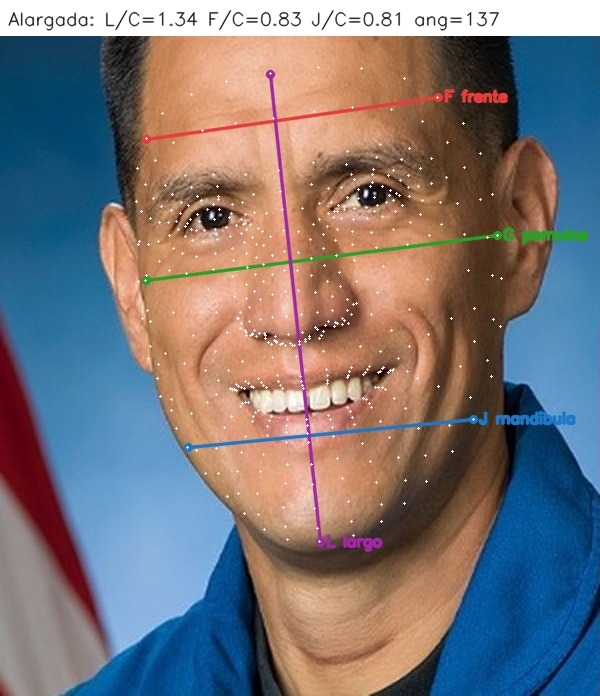
\includegraphics[width=0.42\linewidth]{forma_cara.jpg}
  \caption{Medidas sobre la malla 3D: frente (F), pómulos (C), mandíbula (J) y largo (L). Arriba, las proporciones y la forma resultante.}
  \label{fig:forma}
\end{figure}

\subsection{Barba con plantillas reales}
\label{sec:barba}

La barba no se dibuja desde cero: se ajusta una plantilla real a la cara de la persona.

\textbf{Plantillas.} \archivo{backend/training/harvest_beards.py} recorre CelebAMask-HQ una sola vez y procesa cada foto así:
\begin{enumerate}
  \item filtra por atributos: hombre, sin sombrero, nítida, y clasifica en barba completa, candado, bigote o tres días;
  \item detecta los 68 puntos de la cara;
  \item calcula por píxel un alfa de pelo, ``más oscuro que su entorno'': $\alpha=\operatorname{clip}\big((Y_{\text{local}}-10-Y)/14,0,1\big)$;
  \item descarta las plantillas asimétricas o con poco contraste;
  \item guarda el recorte BGRA, sus puntos y el tono de piel en YCrCb.
\end{enumerate}
Quedan 10 plantillas. En tiempo de ejecución se elige, dentro del estilo pedido, la de croma de piel más cercano al del usuario.

\textbf{Malla.} A los 68 puntos se suman 15 puntos virtuales bajo la mandíbula, para que la barba bajo el mentón quede dentro de la malla. Sobre los 83 puntos se calcula la triangulación de Delaunay con nuestra implementación del algoritmo de Fortune (\archivo{geometry/delaunay_fortune.py}):
\begin{itemize}
  \item una cola de prioridad (\texttt{heapq}) guarda los eventos de sitio y de círculo;
  \item cada evento de círculo aporta directamente un triángulo, sin construir el diagrama de Voronoi completo.
\end{itemize}
También hay una implementación de Bowyer--Watson (\archivo{geometry/delaunay.py}) que da el mismo resultado; se usó para validar.

\textbf{\emph{Warp} afín por triángulo.} \archivo{geometry/warp.py} reemplaza a las funciones de OpenCV por una versión propia. Para cada triángulo:
\begin{enumerate}
  \item resuelve el sistema $3\times3$ de la afín inversa (destino a origen);
  \item recorre los píxeles del rectángulo envolvente del triángulo de destino y se queda con los que tienen coordenadas baricéntricas no negativas;
  \item lee el origen con interpolación bilineal.
\end{enumerate}
Solo se procesan los triángulos cercanos a la barba.

\textbf{Color.} El color del pelo se mide como la mediana dentro de la máscara de pelo y se pasa a YCrCb. A la nube de color de la barba deformada se le suma un desplazamiento constante hacia ese color. Un desplazamiento, y no un reemplazo, conserva la variación interna, es decir, los pelos. El croma se limita a tonos naturales para que un fondo azul no tiña la barba.

\textbf{Región y borde.} La región de cada estilo se arma con polígonos y elipses sobre los 68 puntos:
\begin{itemize}
  \item el bigote es una banda en arco que sigue una curva de Bézier cuadrática;
  \item a la región se le restan los labios y se recorta al casco convexo de la cara;
  \item el borde se suaviza con un \emph{feather} orgánico: distancia al borde (\emph{distance transform}) más ruido.
\end{itemize}

\textbf{Composición en tres capas.} Sea $\rho$ la densidad elegida y $\alpha_r$ el alfa de la región:
\begin{enumerate}
  \item \textbf{cuerpo}: \emph{multiply} con $m=0{,}35+0{,}65\,c/255$ y ruido anisótropo orientado según la dirección del pelo. La luz de la piel sigue viéndose a través de la barba;
  \item \textbf{hebras}: curvas de Bézier cuadráticas que siguen un campo de dirección hacia abajo y hacia afuera. Su cantidad es proporcional a $\rho$, hasta 9000;
  \item \textbf{detalle}: se transfiere solo la alta frecuencia de la plantilla, $\text{plantilla}-G_\sigma(\text{plantilla})$. Así se conservan los pelos reales sin traer el brillo ni el color de la otra persona. Se descartó un \emph{Poisson blending} \cite{perez2003} porque igualaba el brillo con el borde y aclaraba la barba.
\end{enumerate}
El estilo ``tres días'' reemplaza las capas 2 y 3 por un grano de 1~px cuyo umbral baja al subir la densidad. La figura~\ref{fig:barba} muestra los cuatro estilos.

\textbf{En vivo.} La textura se genera una vez y se ancla a la malla de referencia (\texttt{LiveAnchor}):
\begin{itemize}
  \item en cada cuadro, los ruidos se deforman con el mismo \emph{warp};
  \item cada hebra guarda sus coordenadas baricéntricas, de modo que queda pegada a la piel en lugar de ``nadar'' sobre la imagen;
  \item el contraste del grano se restaura después del \emph{warp}, porque interpolar ruido blanco reduce su varianza.
\end{itemize}

\begin{figure}[ht]
  \centering
  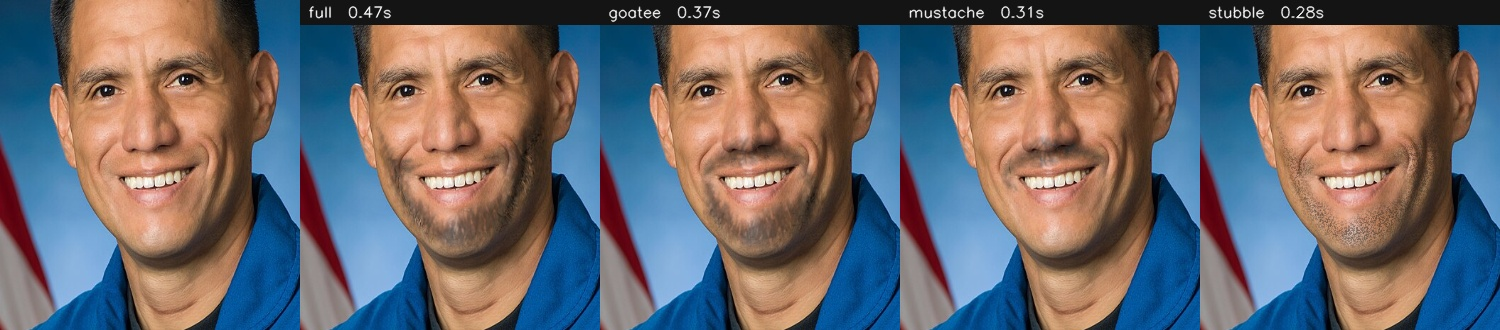
\includegraphics[width=\linewidth]{barba_estilos.jpg}
  \caption{Original y los cuatro estilos de barba sobre un retrato de dominio público: completa, candado, bigote y tres días.}
  \label{fig:barba}
\end{figure}
